\documentclass[tikz,border=10pt]{standalone}
% No extra TikZ libraries are needed for this figure.
\begin{document}
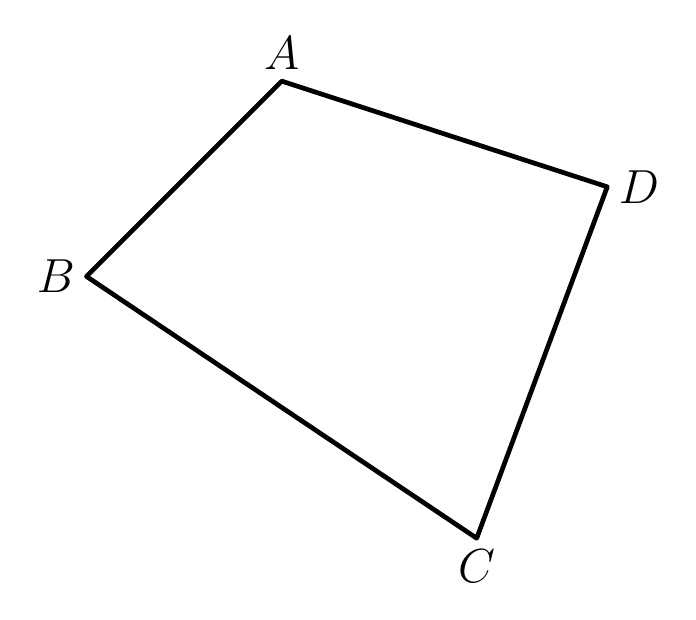
\begin{tikzpicture}[line join=round, line width=1.7pt]
  % Vertices: x = px_x*s, y = (408 - px_y)*s, with s = 0.021108
  \coordinate (A) at (3.958,7.229);
  \coordinate (B) at (1.478,4.749);
  \coordinate (C) at (6.434,1.424);
  \coordinate (D) at (8.092,5.887);

  % Quadrilateral edges AB, BC, CD, DA (solid, black)
  \draw[black] (A) -- (B) -- (C) -- (D) -- cycle;

  % Vertex labels placed outside each vertex
  \node[above] at (A) {\fontsize{17}{20.4}\selectfont $A$};
  \node[left]  at (B) {\fontsize{17}{20.4}\selectfont $B$};
  \node[below] at (C) {\fontsize{17}{20.4}\selectfont $C$};
  \node[right] at (D) {\fontsize{17}{20.4}\selectfont $D$};
\end{tikzpicture}
\end{document}